%%%%%%%%%%%%%%%%%%%%%%%%%%%%%%%%%%%%%%%%%
% Journal Article
% LaTeX Template
% Version 1.4 (15/5/16)
%
% This template has been downloaded from:
% http://www.LaTeXTemplates.com
%
% Original author:
% Frits Wenneker (http://www.howtotex.com) with extensive modifications by
% Vel (vel@LaTeXTemplates.com)
%
% License:
% CC BY-NC-SA 3.0 (http://creativecommons.org/licenses/by-nc-sa/3.0/)
%
%%%%%%%%%%%%%%%%%%%%%%%%%%%%%%%%%%%%%%%%%

%----------------------------------------------------------------------------------------
%	PACKAGES AND OTHER DOCUMENT CONFIGURATIONS
%----------------------------------------------------------------------------------------

\documentclass[twoside,twocolumn]{article}

%\usepackage{booktabs,caption}
\usepackage[flushleft]{threeparttable}
\usepackage{graphicx}
\usepackage{blindtext} % Package to generate dummy text throughout this template 

\usepackage[sc]{mathpazo} % Use the Palatino font
\usepackage[T1]{fontenc} % Use 8-bit encoding that has 256 glyphs
\linespread{1.05} % Line spacing - Palatino needs more space between lines
\usepackage{microtype} % Slightly tweak font spacing for aesthetics

\usepackage[english]{babel} % Language hyphenation and typographical rules

\usepackage[hmarginratio=1:1,top=32mm,columnsep=20pt, left= 2.35cm, right = 2.35cm, footskip = 2cm]{geometry} % Document margins
\usepackage[hang, small,labelfont=bf,up,textfont=it,up]{caption} % Custom captions under/above floats in tables or figures
\usepackage{booktabs} % Horizontal rules in tables

\usepackage{lettrine} % The lettrine is the first enlarged letter at the beginning of the text

\usepackage{enumitem} % Customized lists
\setlist[itemize]{noitemsep} % Make itemize lists more compact

\usepackage{abstract} % Allows abstract customization
\renewcommand{\abstractnamefont}{\normalfont\bfseries} % Set the "Abstract" text to bold
\renewcommand{\abstracttextfont}{\normalfont\small\itshape} % Set the abstract itself to small italic text

\usepackage{titlesec} % Allows customization of titles
\renewcommand\thesection{\Roman{section}} % Roman numerals for the sections
\renewcommand\thesubsection{\roman{subsection}} % roman numerals for subsections
\titleformat{\section}[block]{\large\scshape\centering}{\thesection.}{1em}{} % Change the look of the section titles
\titleformat{\subsection}[block]{\large}{\thesubsection.}{1em}{} % Change the look of the section titles

\usepackage{fancyhdr} % Headers and footers
\pagestyle{fancy} % All pages have headers and footers
\fancyhead{} % Blank out the default header
\fancyfoot{} % Blank out the default footer
%\fancyhead[C]{Running title $\bullet$ May 2016 $\bullet$ Vol. XXI, No. 1} % Custom header text
\fancyfoot[RO,RE]{\thepage} % Custom footer text

\usepackage{titling} % Customizing the title section

\usepackage{hyperref} % For hyperlinks in the PDF

%----------------------------------------------------------------------------------------
%	TITLE SECTION
%----------------------------------------------------------------------------------------

\setlength{\droptitle}{-4\baselineskip} % Move the title up

\pretitle{\begin{center}\huge\bfseries} % Article title formatting
\posttitle{\end{center}} % Article title closing formatting
\title{Studies of Phase Transitions in Magnetic Fields } % Article title

\author{%
\textsc{Andreas Fagerheim}\thanks{\url{https://github.com/AndreasFagerheim/Project-4}} \\[1ex] % Your name
\normalsize Department of Physics, University of Oslo, Norway \\ % Your institution
%\normalsize \href{mailto:john@smith.com}{john@smith.com} % Your email address
%\and % Uncomment if 2 authors are required, duplicate these 4 lines if more
%\textsc{Jane Smith}\thanks{Corresponding author} \\[1ex] % Second author's name
%\normalsize University of Utah \\ % Second author's institution
%\normalsize \href{mailto:jane@smith.com}{jane@smith.com} % Second author's email address
}
\date{\today} % Leave empty to omit a date

%---------------------------------------------------------------------------------------
\renewcommand{\maketitlehookd}{%
\begin{abstract}

This article set forth to examine phase shifts and the critical temperature of materials. This will be done by using the statistical method Ising model. The Ising model implements a algorithm called Metropolis. At a given critical temperature, this model exhbits a phase transition from a magnetic phase (a system with a finite magnetic moment) to a phase with zero magnetization. All programs developed and used are available in the github link in the footnote.


\end{abstract}
}

%----------------------------------------------------------------------------------------

\begin{document}
\maketitle

\section{Introduction}

In the help of understanding phase transition we make use of fluctuations. In physics we make use of statistical models and we will here look closer at the Ising model. The behaviour of said fluctuations can be closer examined using the Isng model and will serve as a tool to better understand the underlying particle interactions. This is a so-called binary system where the objects at each lattice site can only take two values. These could be $-1$ and $1$ or other values.  We can solve the system analytically for certain expectation values in one and two dimensions and it gives a qualitatively  good understanding of several types of phase transitions. The system we will look closer to can be assumed to be a ferromagnetic ordering, viz $J> 0$.  We will use periodic boundary conditions and
the Metropolis algorithm only.

\section{Theory}


\subsection{ Ising Model }
The total energy of the Ising Model can in the simplest form be expressed as

\[
E=-J\sum_{< kl >}^{N}s_ks_l - B \sum_{ k }^{N}s_k
\]
with
$s_k=\pm 1$. The quantity $N$ represents the total number of spins and $J$ is a coupling
constant expressing the strength of the interaction between
neighboring spins.  The symbol $<kl>$ indicates that we sum over
nearest neighbors only. $B$ is an external magnetic field interacting with the magnetic moment set up by the spins \cite{Hjorth-Jensen:2015dg}. This article will look closer at the case of witch there is no interacting external magnetic field and the energy can the be expressed as:
\begin{equation}
E=-J\sum_{< kl >}^{N}s_ks_l
\end{equation}

The expectation value, the mean energy, can be calculated given a probability distribution $P_i$ as
\begin{equation}
\langle E \rangle=  \sum_{i= 1}^{M} E_iP_i(\beta)
\end{equation}
hvor the probability distribution is given by the Boltzmann distribution
\[
P_i(\beta) = \frac{ e^{-\beta E_i}}{Z}
\]
where $\beta = 1/k_bT$ is the inverse temperature, $k_b$ is the Boltzmann constant, $E_i$ is is the energy of a microstate $i$. The partition function is $Z$ and is given for the canonical ensemble as a sum over all microstates, M; 
\[
Z = \sum_{i= 1}^{M} e^{-\beta E_i}.
\]
Further the the expectation values for magnetic moment $|M|$
\begin{equation}
\langle |M| \rangle=  \sum_{i= 1}^{M} M_iP_i(\beta).
\end{equation}
The variance of $E$ and $|M|$ is given receptively as 

\[
 \sigma_E^2 = \langle E^2 \rangle -\langle E \rangle^2
 \]
 \[
 \sigma_M^2 = \langle M^2 \rangle -\langle M \rangle^2
\]
This lets us express the specific heat capacity constant volume as

\begin{equation}
 C_v = \frac{1}{k_bT^2} (\langle E^2 \rangle -\langle E \rangle^2)
\end{equation}

\begin{equation}
 \chi = \frac{1}{k_bT} (\langle M^2 \rangle -\langle M \rangle^2)
\end{equation}
\subsection{ Analytic solutions for the Ising Model of 2x2 lattice }
Looking closer at a 2x2 lattice to find analytical solutions which will serve as a bechmark for the method implemented later with T = 1. \textbf{Table 1} shows the different energies and magnetization states. Using the known states we can find analytical solutions:

\[
Z = \sum_{i= 1}^{M} e^{-\beta E_i} = 2e^{\beta8J}+2e^{-8\beta J}+12e^0.
\]
with $\beta = 1/kT$ and $T = 1$ with unit $kT/J$ we get:
\[
Z = 2e^{8}+2e^{-8}+12e^0.
\]
\begin{table}[h]
  \begin{threeparttable}
    \caption{The different energy states of the 2x2 Ising Model}
     \begin{tabular}{lllll}
        \toprule
        No. of spins & Degeneracy & Energy & Magnetization &  \\
        \midrule
                
        4    & 1        & -8J   & 4       	   \\
        3    & 4        &  0    & 2          \\
        2    & 4        &  0    & 0          \\
        2    & 2        &  8J   & 0          \\
        1    & 4        &  0    & -2          \\
        0    & 1        & -8J   & -4          \\
        \bottomrule
     \end{tabular}
    \begin{tablenotes}
      \small
      \item Showing the different energy and magnetization for the two-dimensional Ising model with periodic boundary conditions.
    \end{tablenotes} 
  \end{threeparttable}
  
\end{table}

This gives us the energy
\begin{equation}
\langle E \rangle=  \sum_{i= 1}^{M} E_iP_i(\beta) =\frac{1}{Z} \sum_{i= 1}^{M} E_ie^{-\beta E_i}
\end{equation}
\[
\langle E \rangle=  \frac{1}{Z}(-8e^8 +8e^{-8} +8e^{-8}-8e^{8}) = -7.9839
\]
\[
\frac{\langle E \rangle}{N}= -1.99598
\]
hvor $N = 4$. In the same way the magnetization turns out to be

\begin{equation}
\langle |M|\rangle=  \frac{1}{Z}\sum_{i= 1}^{M} M_i e^{E_i} = 3.9946
\end{equation}
\[
\frac{\langle |M| \rangle}{N}= 0.9986
\]
The heat capacity then becomes:
\begin{equation}
\langle E^2 \rangle= \frac{1}{Z} \sum_{i= 1}^{M} E_i^2e^{E_i}= \frac{128e^8+128e^{-8}}{5973.917}
\end{equation}
\[
\frac{C_V}{N} = \frac{\langle E^2 \rangle -{\langle E \rangle}^2}{4}= 0.12832 = 0.03208
\]
The magnetic susceptibility  can in the same way be calculated to $\frac{\chi}{N} = 0.00401$.


\subsection{Studies of phase transitions.}


For many materials there exist a critical temperature, $T_C$, at which the material changes its characteristics and undergoes a phase transition. In this case the Ising model can give us a tool for examination of the characteristics. The mean magnetization can for the Ising model be expressed:
As an example, for the Ising class of models, 
the mean magnetization is given by
\[
  \langle M(T) \rangle \sim \left(T-T_C\right)^{\beta},
\]
where $\beta=1/8$ is a so-called critical exponent. For the heat capacity and the magnetic susceptibility  it can in the same way be expressed as

\[
  C_V(T) \sim \left|T_C-T\right|^{\alpha},
\]

\begin{equation}
  \chi(T) \sim \left|T_C-T\right|^{\gamma},
\end{equation}
with $\alpha = 0$ and $\gamma = 7/4$.

A second-order phase transition is characterized by a
correlation length. The behavior at finite lattice can be related the results for an infinite lattice. Scaling of the critical temperature take the form


\begin{equation}
 T_C(L)-T_C(L=\infty) = aL^{-1/\nu},
 \label{eq:tc}
\end{equation}

with  $a$ a constant and  $\nu$ defined in Eq. (11). 
We set $T=T_C$ and obtain a mean magnetisation

\begin{equation}
  \langle {\cal M}(T) \rangle \sim \left(T-T_C\right)^{\beta}
  \rightarrow L^{-\beta/\nu},
  \label{eq:scale1}
\end{equation}
a heat capacity

\begin{equation}
  C_V(T) \sim \left|T_C-T\right|^{-\gamma} \rightarrow L^{\alpha/\nu},
  \label{eq:scale2}
\end{equation}
and susceptibility

\begin{equation}
  \chi(T) \sim \left|T_C-T\right|^{-\alpha} \rightarrow L^{\gamma/\nu}.
  \label{eq:scale3}
\end{equation}
\section{Metropolis algorithm}
The Metropolis algorithm builds on the principle of natures desire to reach equlibrum towards lower energy levels. Simply explained it starts of by picking a random place in the spin matrix. It then try to flip the spin if the calculated change in energy is making the total energy lower in the system. Flipping the spin is then thougt to make the system closer to equilibrium.

%------------------------------------------------

\section{Results}

From \textbf{Table 1} we see that the numerical value of $E$ compared to the analytical value for the 2 x 2 lattice, and some other values. \textbf{Figure 2} shows how the Energy develops with the increasing number of Monte Carlo cycles. Here we see that after 40000 cycles the values fluctuates less and is close to the analytical solution. The same can be said about the mean magnetization shown in the lower plot in \textbf{Figure 1}.
\\
\\
\\
\\
\\

\begin{table}
\begin{tabular}{|l|l|l|l|l|}
\hline
MC cycles &  ${E}/{N}$   & ${C_V}/{N}$    & ${|M|}/{N}$      & $ \chi/{N} $     \\ \hline
Analytisk & -1.9959 & 0.03208   & 0.9986   & 0.00401  \\ \hline
20000     & -1.9951 & 0.03910 & 0.9983 & 0.005288 \\ \hline
40000     & -1.9966 & 0.02755 & 0.9988 & 0.003669 \\ \hline
60000     & -1.9966 & 0.02715 & 0.9988 & 0.003345 \\ \hline
80000     & -1.9964 & 0.02875 & 0.9987 & 0.003707 \\ \hline
100000    & -1.9966 & 0.02699 & 0.9989 & 0.003455 \\ \hline
\end{tabular}
\caption{Comparison of the analytical values and the numerical values with increasing number of Monte Carlo cycles.}
\label{tab:my-table}

\end{table}
\begin{figure}[h]
  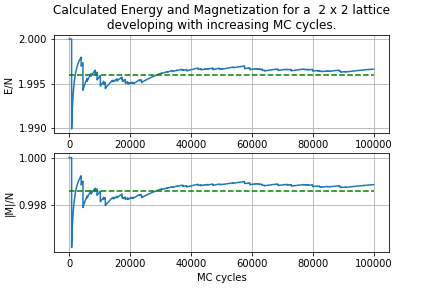
\includegraphics[width= 10cm]{N=2T=1.png}
  \caption{Energy and magnetization as a function of Monte Carlo cycles. The plot is for a 2 x 2 lattice and with the initial temperature set to $k_bT/J = 1$. }
  \label{fig:boat1}
\end{figure}


For a lattice of dimensions 20 X 20 the development of energy and mean magnetisation as a function of Monte Carlo cycles is plotted in figure 2,3,4,5. It is evident that the system reaches a state of  equilibrium already around 20 000 cycles. 

\begin{figure}[h]
  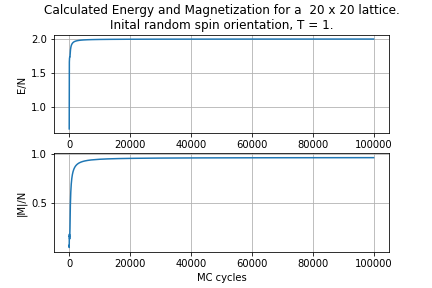
\includegraphics[width= 10cm]{N=20T=1R.png}
  \caption{Energy and magnetization as a function of Monte Carlo cycles. The plot is for a 20 x 20 lattice and with the initial temperature set to $k_bT/J = 1$ and an initial random spin orientation.}
  \label{fig:boat2}
\end{figure}

\begin{figure}[h]
  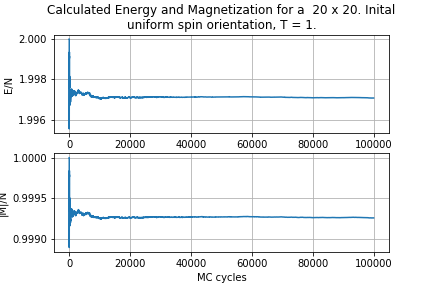
\includegraphics[width= 10cm]{N=20T=1U.png}
  \caption{Energy and magnetization as a function of Monte Carlo cycles. The plot is for a 20 x 20 lattice and with the initial temperature set to $k_bT/J = 1$ and an initial uniform spin orientation.}
  \label{fig:boat3}
\end{figure}

\begin{figure}[h]
  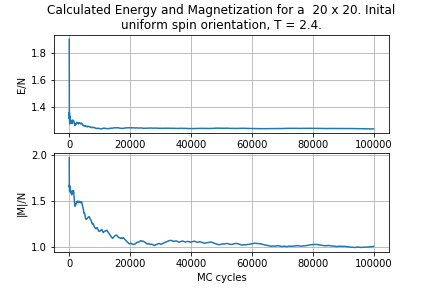
\includegraphics[width= 10cm]{N=20T=2.4U.png}
  \caption{Energy and magnetization as a function of Monte Carlo cycles. The plot is for a 20 x 20 lattice and with the initial temperature set to $k_bT/J = 2.4$ and an initial random spin orientation.}
  \label{fig:boat4}
\end{figure}

\begin{figure}[h]
  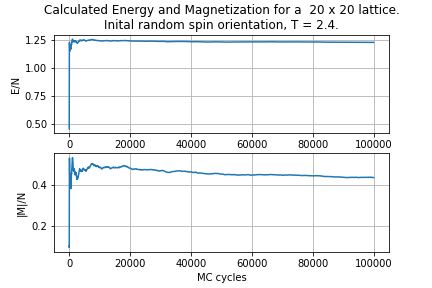
\includegraphics[width= 10cm]{N=20T=2.4R.png}
  \caption{Energy and magnetization as a function of Monte Carlo cycles. The plot is for a 20 x 20 lattice and with the initial temperature set to $k_bT/J = 2.4$ and an uniform random spin orientation.}
  \label{fig:boat5}
\end{figure}

Looking at figure 6 and 7 should give and indication on how the number of accepted states should develop with the increasing number of cycles. Number of accepted configurations seems to increase with the temperature.There should although be said that the numbers in fig 7 don't makes sense i the magnitude nesseceraly, but the number of states should behave in the same way as the number of cycles increase. The initial spin orientation does not affect the number of possible configurations after some time has passed. Temperature does seem to increase the number of acceptable states per cycle, but i don't know if by as much as the results indicates. This aligns with the principal that with higher temperature, the probability for accepting a state increases.
\\
\\
\\
\\
\\

\begin{figure}[h]
  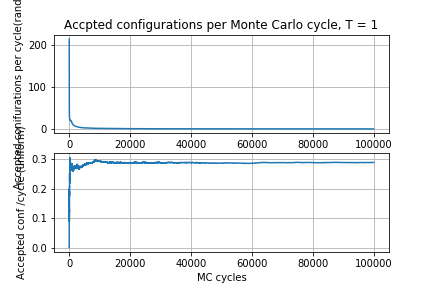
\includegraphics[width= 10cm]{acceptedConfigsT1.png}
  \caption{Energy and magnetization as a function of Monte Carlo cycles. The plot is for a 20 x 20 lattice and with the initial temperature set to $k_bT/J = 2.4$ and an uniform random spin orientation.}
  \label{fig:boat6}
\end{figure}

\begin{figure}[h]
  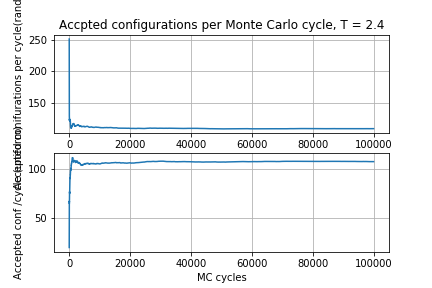
\includegraphics[width= 10cm]{acceptedConfigsT2.png}
  \caption{Energy and magnetization as a function of Monte Carlo cycles. The plot is for a 20 x 20 lattice and with the initial temperature set to $k_bT/J = 2.4$ and an uniform random spin orientation.}
  \label{fig:boat7}
\end{figure}

\subsection{Probability}
Looking at \textbf{Figure 8} and \textbf{Figure 9}. For the case $T = 2.4$ the distribution favours towards the right, which is towards the origin. This coincides with the Boltzmann distribution.


\begin{figure}[h]
  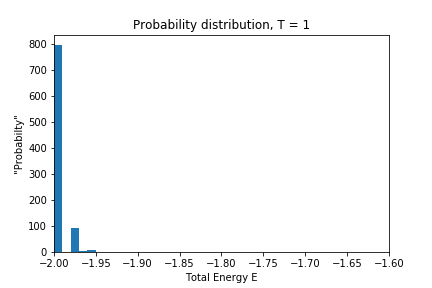
\includegraphics[width= 10cm]{probdist1.png}
  \caption{Probability distribution for a 20 x 20 lattice and with the initial temperature set to $k_bT/J = 1$ .}
  \label{fig:boat8}
\end{figure}

\begin{figure}[h]
  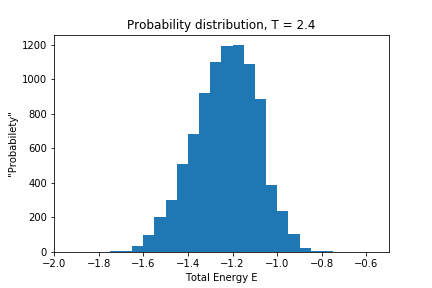
\includegraphics[width= 10cm]{probdist2.png}
  \caption{Probability distribution for a 20 x 20 lattice and with the initial temperature set to $k_bT/J = 2.4$ .}
  \label{fig:boat8}
\end{figure}












\section{Conclusion}
The Ising model has given us a taste of some of the characteristichs the system undergoes. The system clearly reaches an equlibrum and the temperature can bee seen to impact the system. With a higher inital temperature of the system there will be a higher number of possible microstates. The analytucal solutions of the 2x2 lattice serves as a way of validating the method and insight to how it works.
%----------------------------------------------------------------------------------------
%	REFERENCE LIST
%----------------------------------------------------------------------------------------

\begin{thebibliography}{99} % Bibliography - this is intentionally simple in this template
%A statement requiring citation \cite{Hjorth-Jensen:2015dg}.
\bibitem[Hjorth-Jensen, 2015]{Hjorth-Jensen:2015dg}
Hjort-Jensen, M. (2015).
\newblock Computational Physics.
\bibitem[Hjorth-Jensen]{Hjorth-Jensen}
Hjort-Jensen, M.
\newblock https://github.com/CompPhysics/ComputationalPhysics

 
\end{thebibliography}

%----------------------------------------------------------------------------------------

\end{document}
